% Chapter Template

\chapter{Ensayos y resultados} % Main chapter title
En este capítulo se detallan los ensayos realizados en las formaciones ferroviarias y en los talleres de Trenes Argentinos. El orden cronológico de los ensayos es distinto al del desarrollo del firmware. En este documento se ha presentado previamente el diseño de la solución para facilitar la comprensión del trabajo realizado. El desarrollo de la solución fue posterior a una serie de mediciones realizadas en los talleres que permitieron identificar parámetros clave del sistema. \\

En las secciones que siguen se explican las mediciones realizadas en las visitas a los talleres de Victoria y Castelar de Trenes Argentinos Operaciones. Luego se presenta un análisis de datos de las tramas relevadas y también las pruebas de integración propuestas para validar el desarrollo. \\


\label{Chapter4} % Change X to a consecutive number; for referencing this chapter elsewhere, use \ref{ChapterX}

%----------------------------------------------------------------------------------------
%	SECTION 1
%----------------------------------------------------------------------------------------

\section{Mediciones}

\section{Análisis de tramas}

\section{Pruebas en maqueta}

En el circuito esquemático de la figura \ref{fig:schDriverled} se presenta el detalle de conexiones eléctricas entre bloques. Se puede observar que a la salida del conector de datos (CONN 2x8) hay dos buffers de la serie 74HC245D que direccionan las señales eléctricas a izquierda y derecha del arreglo de matrices led. A izquierda viajan las señales SER(data), SRCLK (Clock) y XXX (latch) al arreglo de Shift Registers de la serie 74HC595. Por la derecha se maneja la habilitación secuencial de las filas a través de un arreglo de decodificadores 3x8 de la serie 74HC138. Cada salida de los decodificadores se conecta a un driver de corriente en arreglo de transistores MOSFET FDS4953. Estos decodificadores cableados adecuadamente permiten manejar las 32 señales de un cartel de 4x8 módulos led. \\
%
%
%\begin{figure}[ht]
%	\centering
%	%\includepdf[pages={1}, angle=90]{./Figures/output.driverled.pdf}
%	\includegraphics[width=1.66\textwidth, angle=90]{./Figures/output.driverled.pdf}
%	\caption{Circuito esquemático de la placa controladora de los carteles de matriz led.}
%	\label{fig:schDriverled}
%\end{figure}


\begin{figure}[ht]
	\centering
	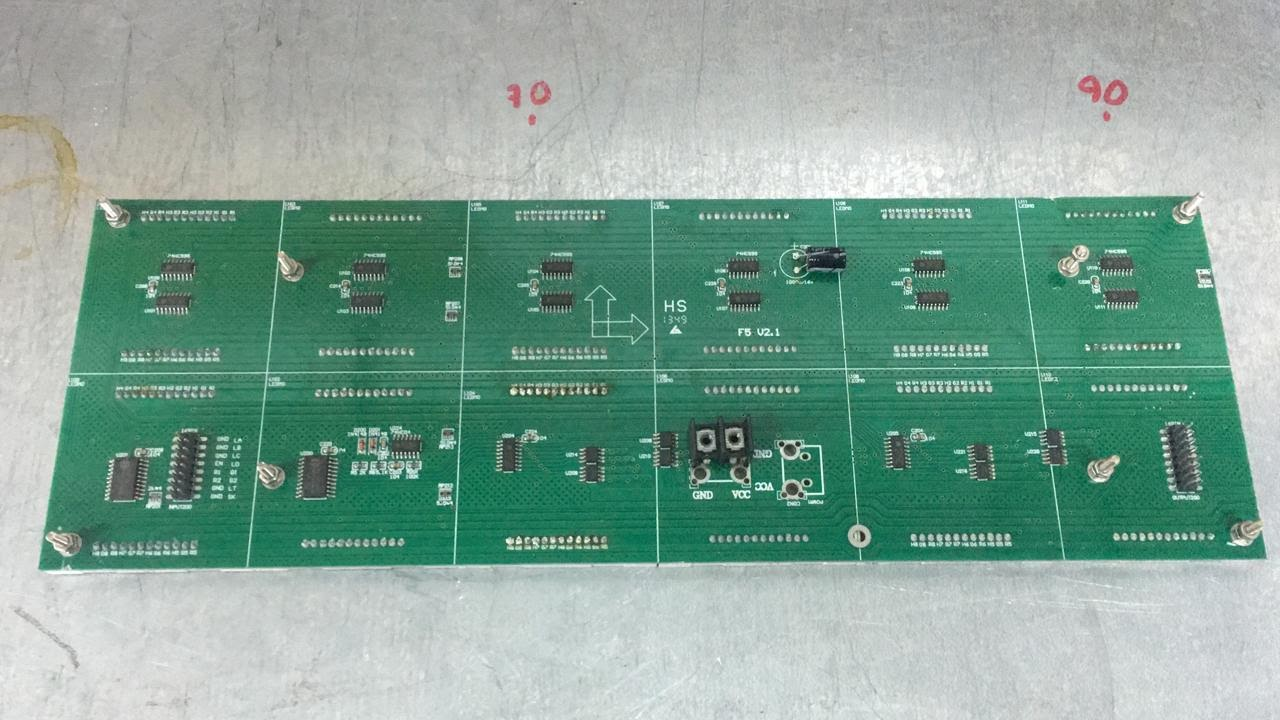
\includegraphics[width=1\textwidth]{./Figures/cartel2x6.jpeg}
	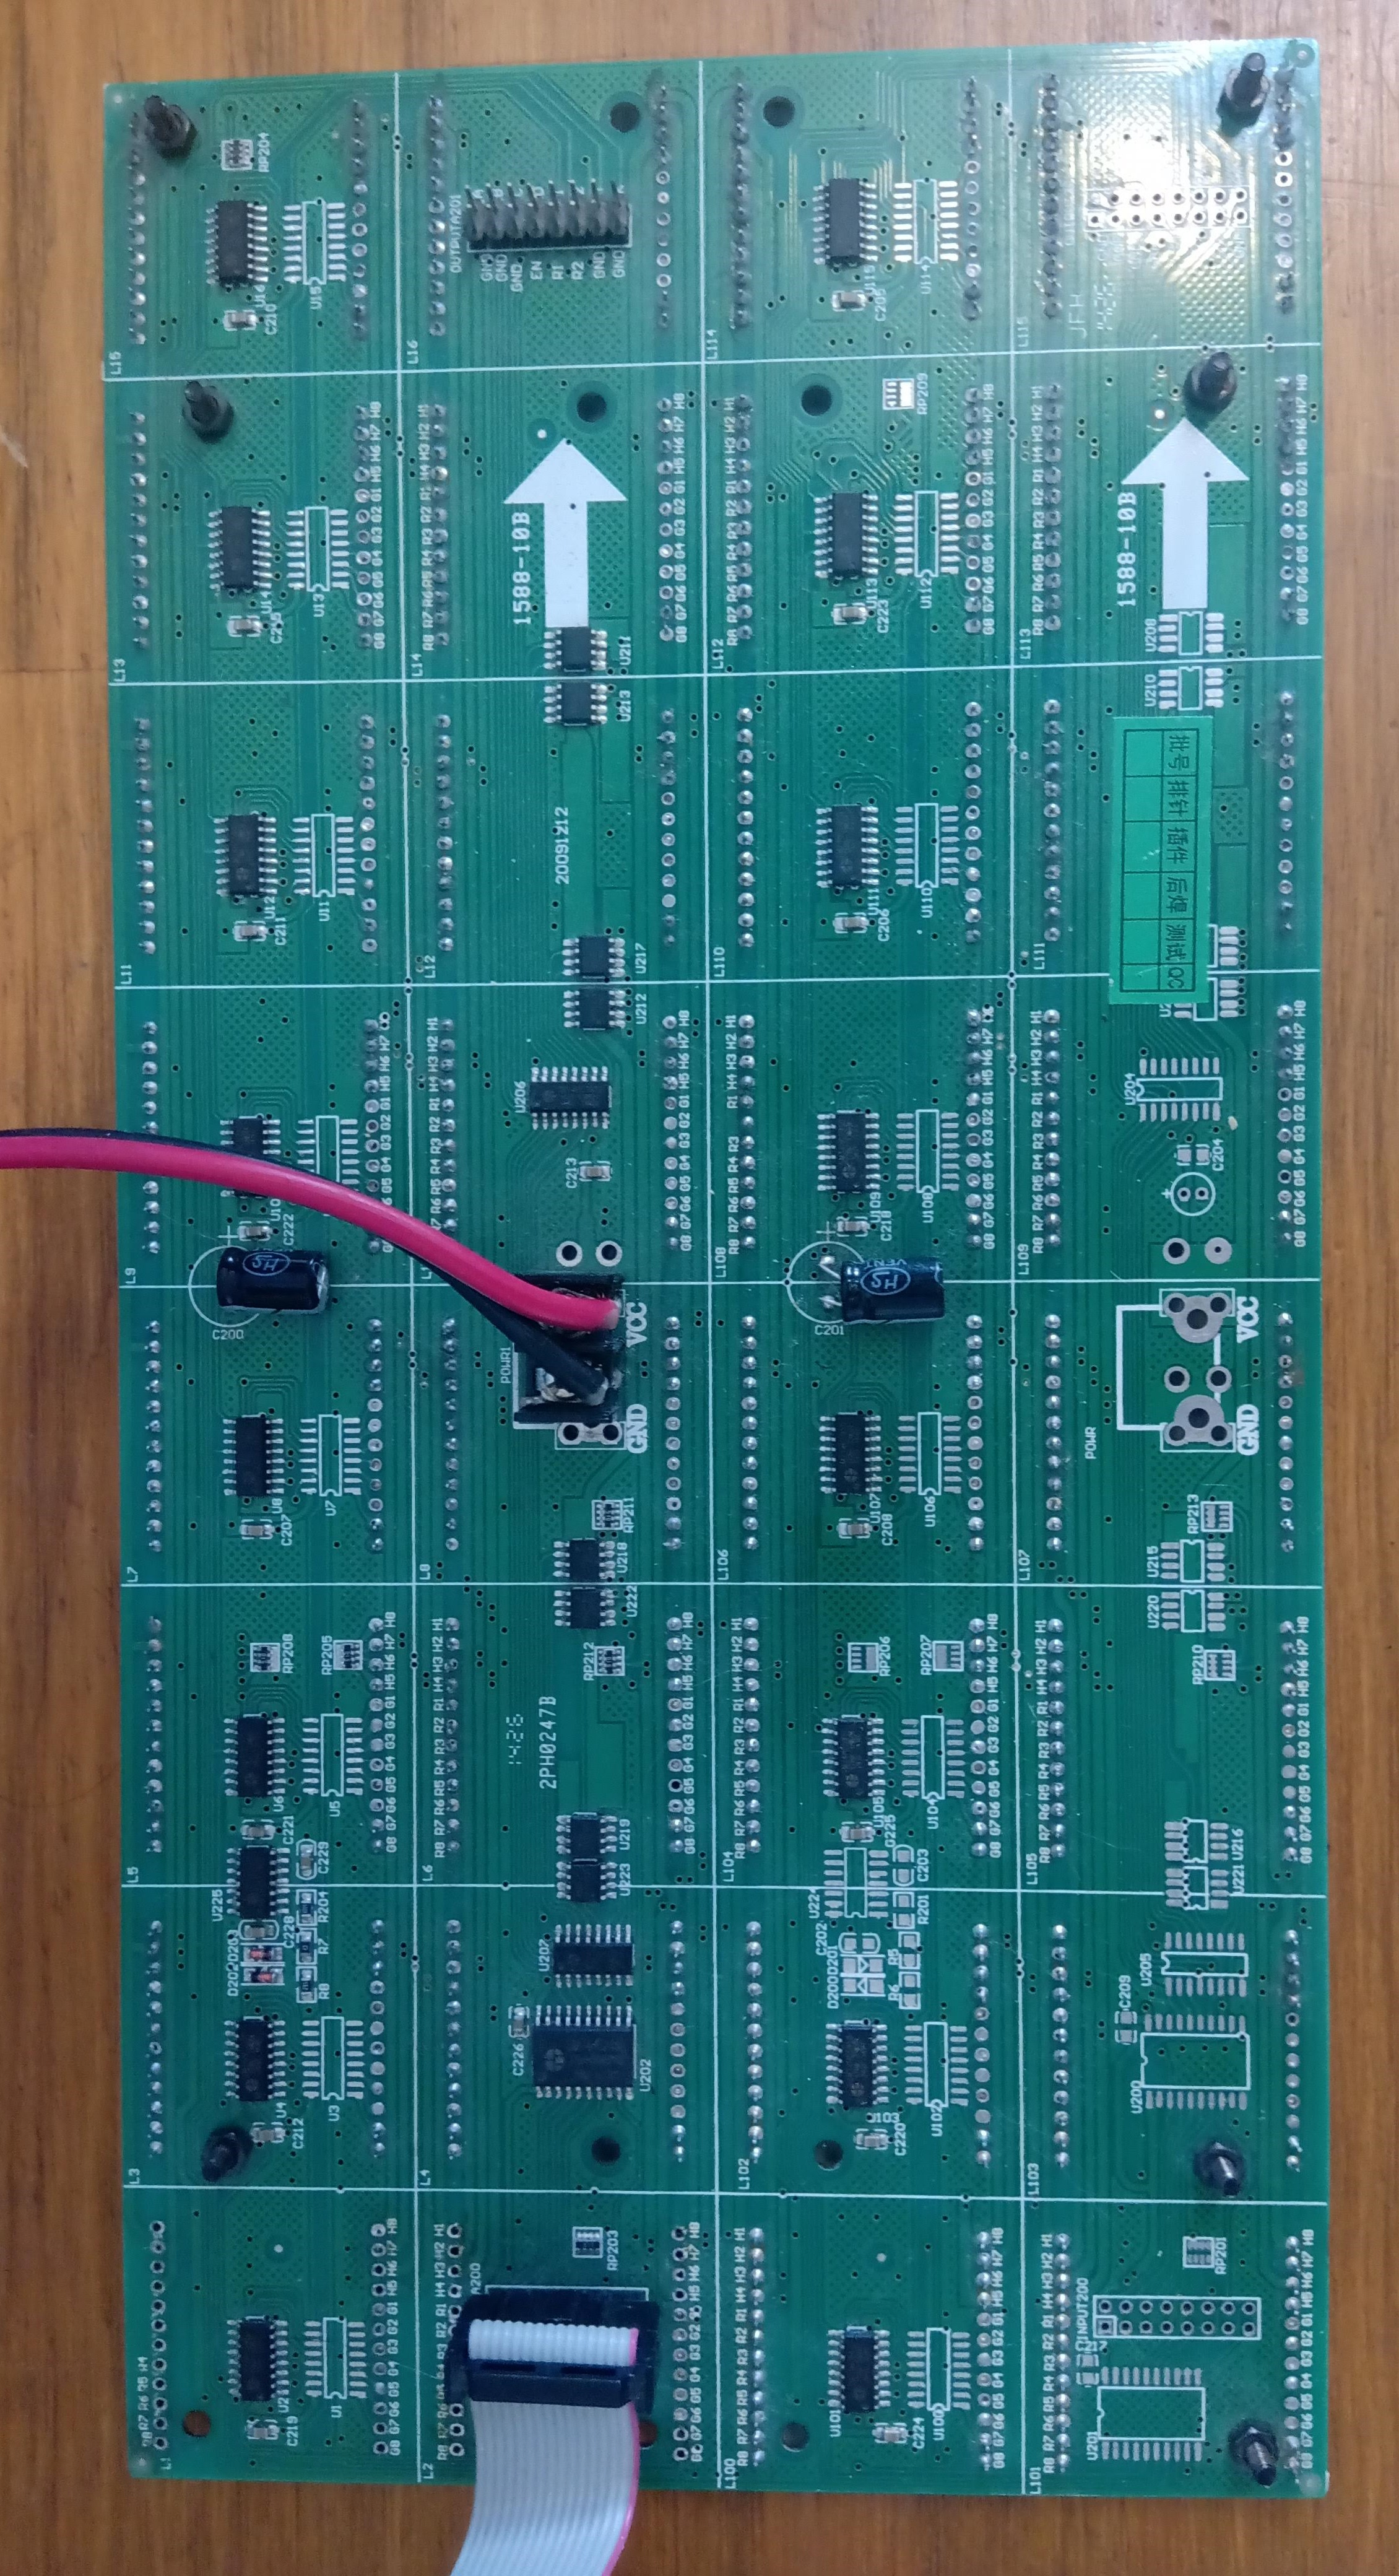
\includegraphics[width=0.75\textwidth, angle=270]{./Figures/cartel4x8.jpg}\\
	\includegraphics[width=1\textwidth]{./Figures/cartelledON.jpg}\\
	\caption{Fotografías de placas de control de los carteles de matriz led: (a) placa de 2x6 módulos; (b) placa de 4x8 módulos; (c) vista posterior de la placa de 4x8.}
	\label{fig:picsDriverled}
\end{figure}


\subsubsection{Placa de control}

\begin{figure}[ht]
	\centering
	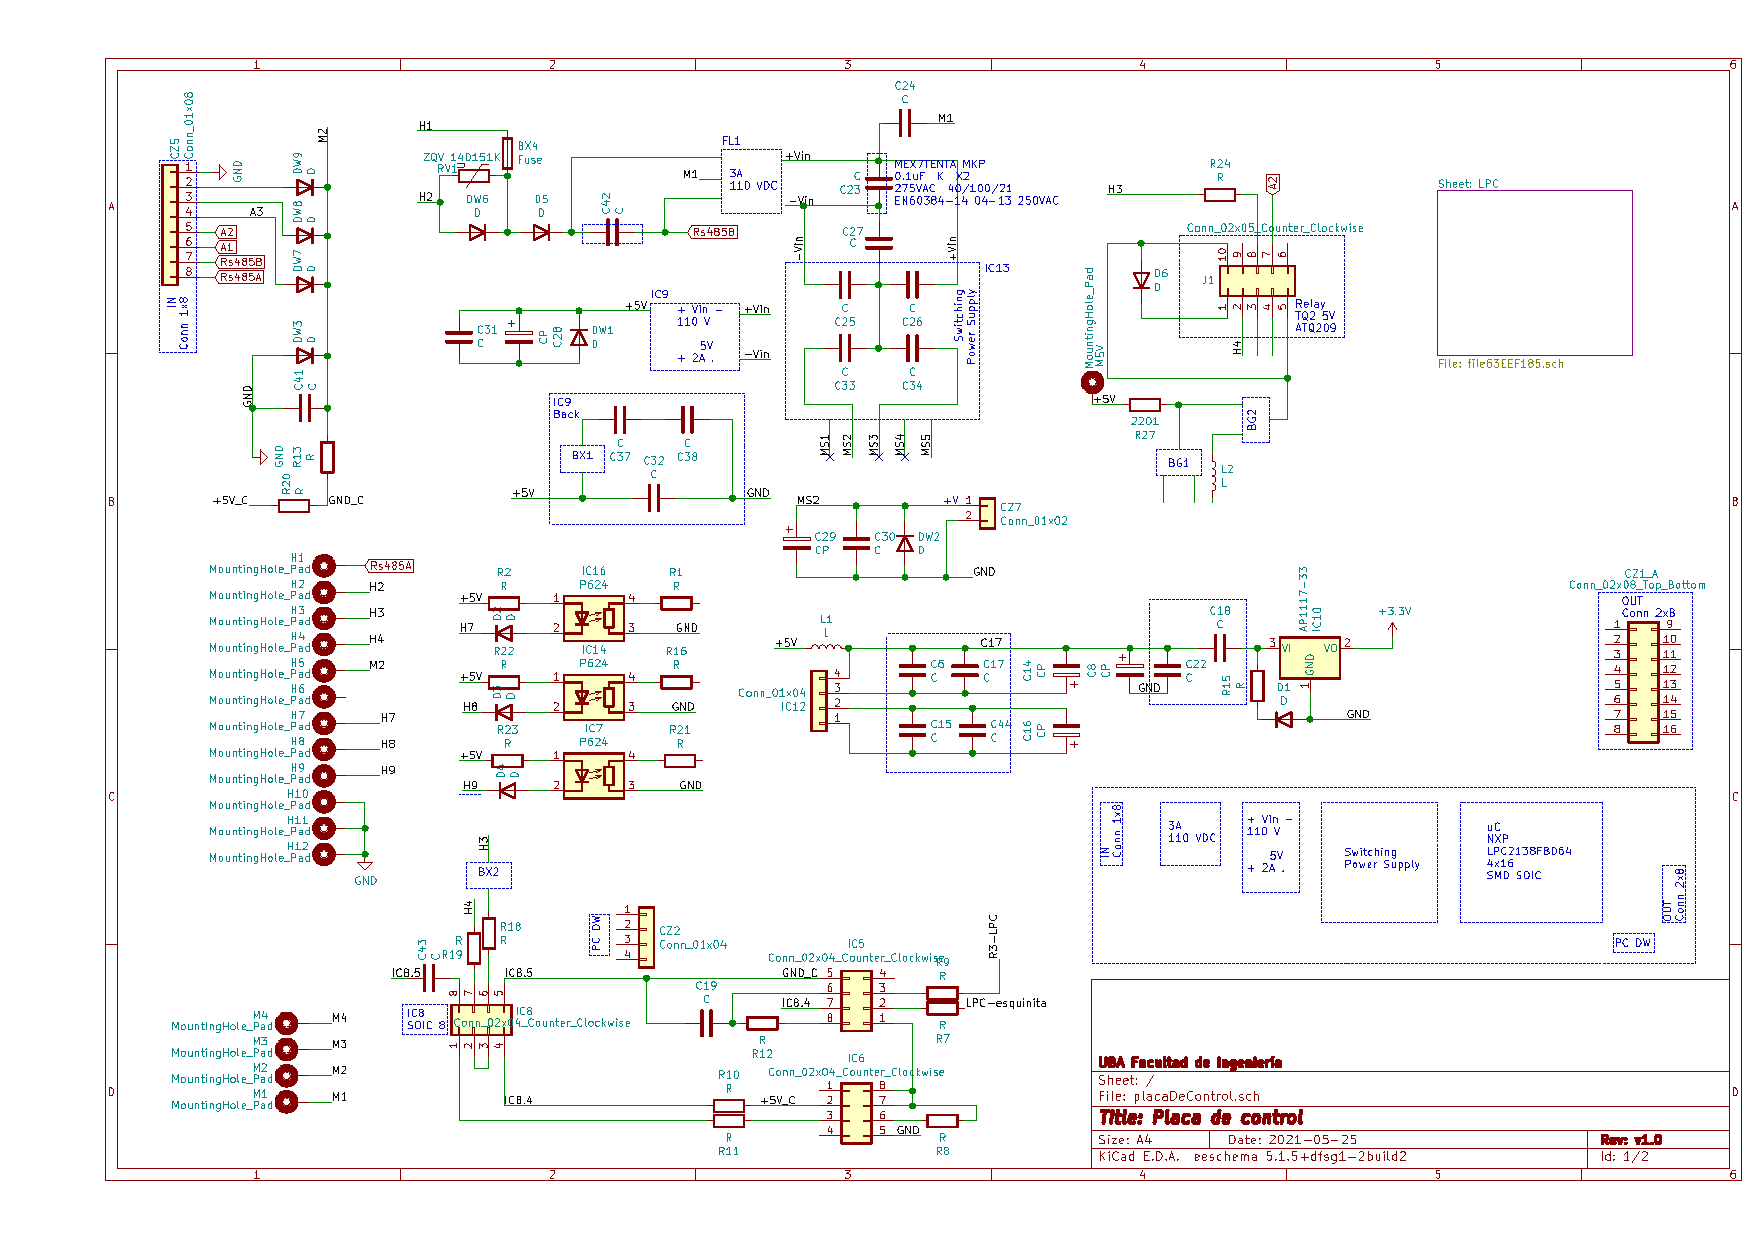
\includegraphics[width=1\textwidth]{./Figures/output.placaControl.pdf}
	\caption{Circuito esquemático de la placa de control de los carteles LED de salón.}
	\label{fig:schController}
\end{figure}


\begin{figure}[ht]
	\centering
	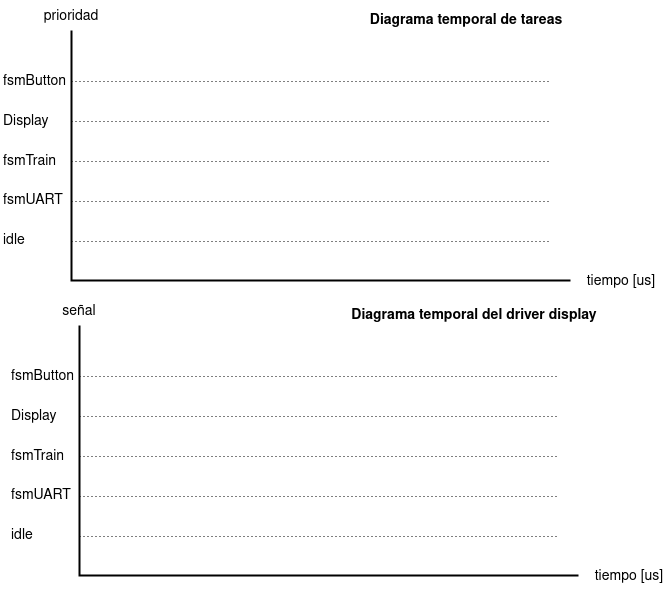
\includegraphics[width=0.5\textwidth]{./Figures/diagramasTemporales.png}
	\caption{}
	\label{fig:diagramasTemporales}
\end{figure}

\section{Integración con red PIDS}

\section{Pruebas de campo}

\begin{figure}[ht]
	\centering
	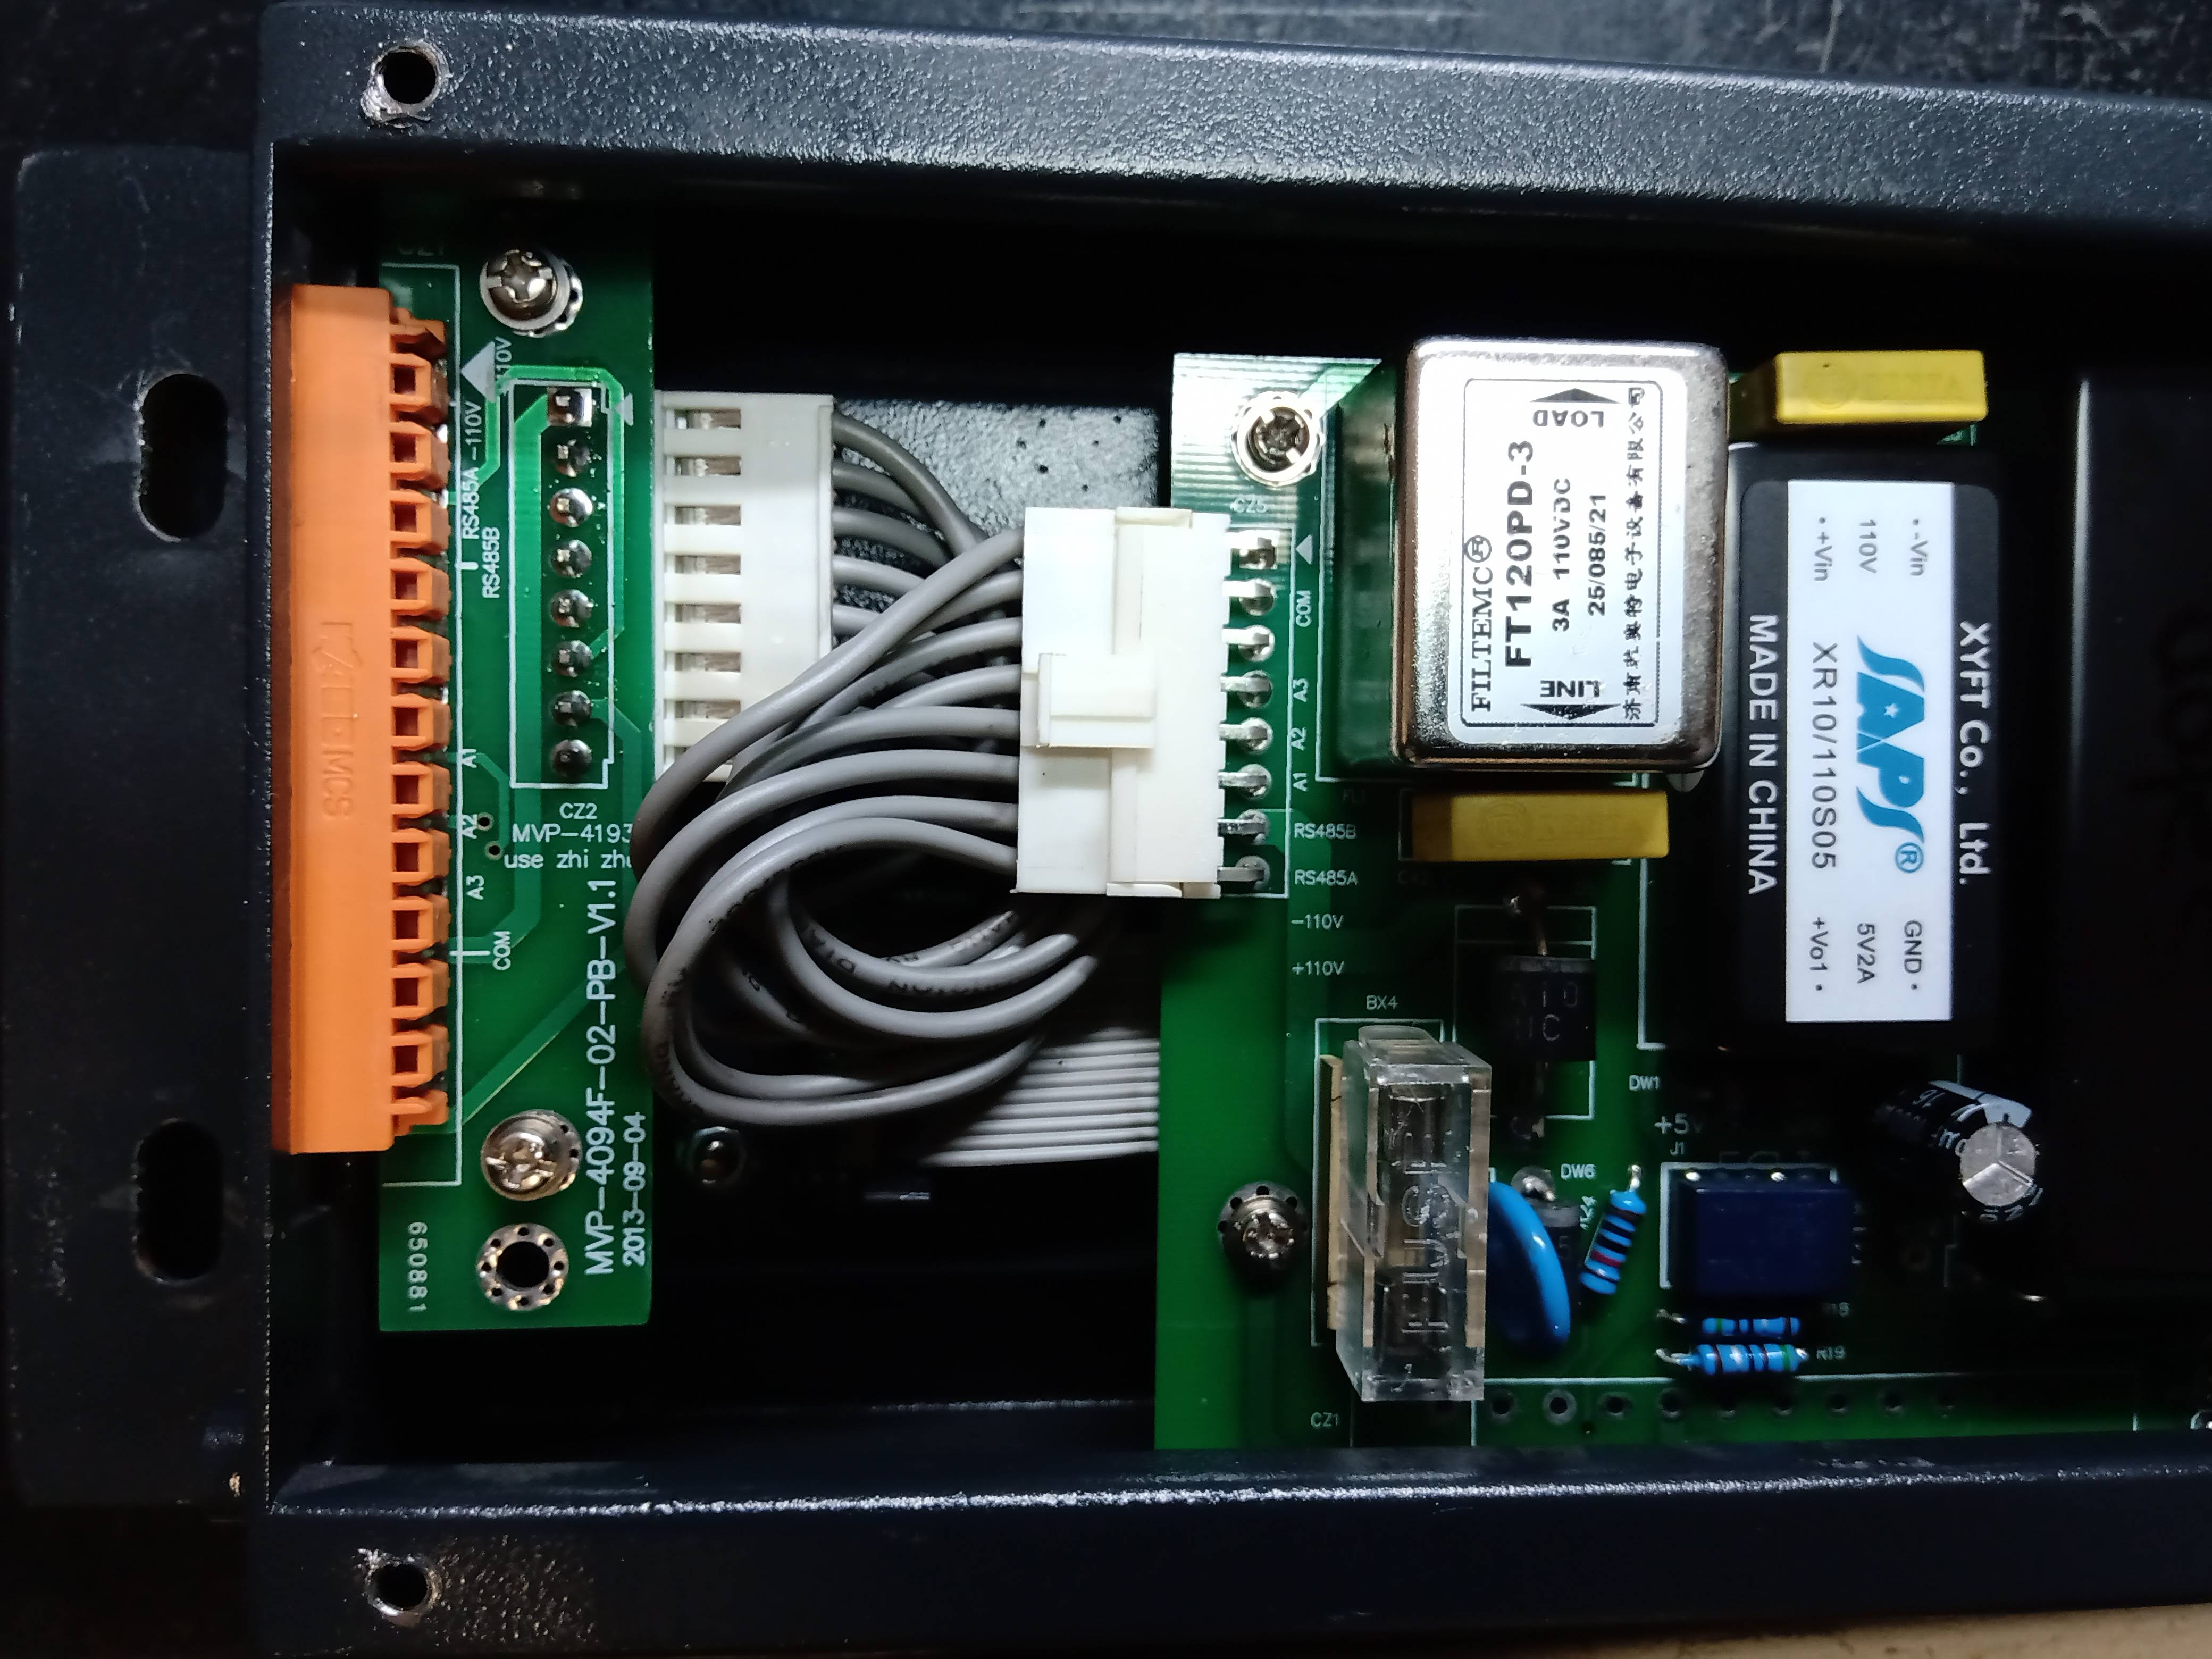
\includegraphics[width=1\textwidth]{./Figures/displayController.jpg}
	\caption{Fotografía del detalle de conexión de la placa de control de los carteles led de salón.}
	\label{fig:displayController}
\end{figure}